\documentclass[
  aps,
  prd,
  superscriptaddress,
  nofootinbib,
  longbibliography,
  12pt
]{revtex4-2}

\usepackage[T1]{fontenc}
\usepackage[utf8]{inputenc}
\usepackage{amsmath,amssymb,bm,mathtools}
\usepackage{booktabs}
\usepackage{graphicx}
\usepackage{xcolor}
\usepackage{hyperref}
\usepackage[nameinlink,capitalise]{cleveref}

\hypersetup{
  colorlinks=true,
  citecolor=blue!55!black,
  linkcolor=blue!55!black,
  urlcolor=blue!55!black
}

\newcommand{\dd}{\mathop{}\!\mathrm{d}}
\newcommand{\E}{\mathbb{E}}
\newcommand{\Var}{\operatorname{Var}}
\newcommand{\SE}{\operatorname{SE}}
\newcommand{\R}{\mathbb{R}}
\newcommand{\Lcal}{\mathcal{L}}
\newcommand{\Pois}{\operatorname{Pois}}
\newcommand{\Normal}{\mathcal{N}}
\newcommand{\pRef}{p_{\mathrm{ref}}}
\newcommand{\qRef}{q_{\phi}}
\newcommand{\rhat}{\widehat r}
\newcommand{\muhat}{\widehat\mu}

\begin{document}

\title{A hybrid neural simulation-based inference method for LHC analyses}

\author{Rafael Coelho Lopes de S\'a}
\affiliation{Department of Physics, University of Massachusetts, Amherst, Amherst 01003, USA}
\author{Jay Sandesara}
\affiliation{Data Science Institute, University of Wisconsin--Madison, Madison, Wisconsin 53706, USA}

\date{\today}

\begin{abstract}
Classifier estimates of density ratios have made high-dimensional, unbinned neural simulation-based inference practical for LHC analyses.  A ratio-only formulation, however, provides neither an explicit normalized density nor a direct generative model, so expected-data calculations and Neyman constructions rely on large finite simulated samples.  Normalizing flows provide normalized densities and efficient sampling, but small absolute-density errors can bias the inference of a small signal in a much larger background.

We propose \emph{hybrid neural simulation-based inference}.  A flow is trained on a balanced, physically representative reference distribution, and events from that learned reference form the denominator sample for classifier estimates of every process-to-reference ratio.  Each process density is the tractable reference-flow density multiplied by its learned ratio.  This division of labor preserves discriminative ratio precision while making the complete event intensity tractable and sampleable.  We derive a weighted, unbinned Asimov construction and train a second flow as a neural importance proposal for its expected likelihood-ratio scan.  In a five-dimensional small-signal demonstration, the finite Asimov sample fits exactly at its generating value and predicts the estimator and discovery-statistic distributions observed in pseudo-experiments.  Neural importance sampling reduces the discovery-statistic variance by a factor of $2.69$ at fixed sample size and the full-scan RMSE by $39\%$.  The reference flow makes Asimov inference cheap and renewable; neural importance sampling makes it efficient.
\end{abstract}

\maketitle

\section{Introduction}
\label{sec:introduction}

Likelihood-based measurements at the Large Hadron Collider (LHC) conventionally compress reconstructed events into one or a few binned observables.  This construction is robust and computationally convenient, but the compression and binning can discard information when the likelihood depends nonlinearly on parameters or when no low-dimensional summary is sufficient over the full parameter space.  Neural simulation-based inference (NSBI) instead uses high-dimensional simulated events to estimate likelihoods or likelihood ratios directly in reconstructed feature space~\cite{Cranmer:2015bka,Brehmer:2018eca,Brehmer:2018hga}.

The ATLAS Collaboration developed a practical classifier-based NSBI formalism for LHC parameter estimation~\cite{ATLAS:2024rpr}.  It was deployed in the measurement of off-shell Higgs-boson production in the $H^{*}\!\to ZZ\to4\ell$ final state~\cite{ATLAS:2024tgo}.  The formalism uses neural estimates of density ratios together with an analytic factorization of the dependence on parameters of interest (POIs) and nuisance parameters.  It can therefore describe dozens of POIs and hundreds of nuisance parameters without densely sampling that complete parameter space during network training.  We refer to this construction as \emph{semi-parametric NSBI}; it is also commonly described as parametrized or factorized NSBI~\cite{Sandesara:2026lectures}.

Density ratios are sufficient for inference based on a profile likelihood ratio.  They are also often easier to estimate to the required precision than absolute densities.  A reference sample can be designed to resemble the relevant physics, sharing resonant structure, tails, and detector effects with the target samples.  The resulting ratios vary more mildly than either absolute density, and they can be learned discriminatively with a binary cross-entropy objective.  This numerical advantage was central to the precision achieved in the ATLAS studies.

A ratio-only representation nevertheless has an operational limitation: it is not itself a generative density model.  An unbinned Asimov dataset must be approximated by a large weighted Monte Carlo (MC) sample, and pseudo-experiments must be constructed by resampling such a sample.  The former makes repeated profiling and impact calculations costly; the latter requires an MC pool much larger than a typical pseudo-experiment~\cite{ATLAS:2024rpr}.  These difficulties do not invalidate ratio-based inference, but they make some standard LHC statistical workflows expensive.

Normalizing flows address the complementary problem.  They provide both a normalized, tractable density and efficient event generation~\cite{Rezende:2015flows,Dinh:2016realnvp,Durkan:2019splines,Papamakarios:2019flows}.  The difficulty is precision: two separately trained process flows can each pass many marginal checks while their residual, unrelated absolute-density errors bias the process-density ratio that controls a small-signal measurement.  Recent work has developed factorized parameter-dependent flows~\cite{Valsecchi:2026flows}, but the required absolute-density accuracy remains a central question when the signal is orders of magnitude smaller than the background.

This paper combines the two representations.  A flow supplies a normalized, sampleable reference density, while classifiers learn the precision-critical ratios of every process to that exact learned reference.  The reference flow is a proposal distribution, not an uncorrected model of each process.  If the ratio estimators are exact, local reference-flow error cancels algebraically.  What the flow must provide is common support and efficient coverage.  The resulting \emph{hybrid NSBI} construction supplies a tractable likelihood, direct weighted or resampled event generation, and a deterministic unbinned Asimov measure.

The same formulation exposes the Asimov calculation as numerical integration.  Direct samples from the reference flow make this integration inexpensive and remove the resolution limit of a finite MC pool, but ordinary Monte Carlo still converges as $M^{-1/2}$.  We therefore train a second flow as a neural importance proposal for the complete expected test-statistic scan.  This distinction is useful in practice: the reference flow makes an Asimov dataset \emph{cheap}, because additional independent quadrature points can be produced on demand; the importance proposal makes it \emph{efficient}, because fewer points are required for a target precision.

The remainder of this paper is organized as follows.  \Cref{sec:semiparametric} reviews semi-parametric NSBI and its practical limitations.  \Cref{sec:hybrid} introduces the hybrid density and sampling construction.  \Cref{sec:asimov} derives the weighted unbinned Asimov likelihood and its finite-sample uncertainty, including the precise role of a flow reference.  \Cref{sec:efficient-asimov} discusses variance-reduced flow quadratures and develops neural importance sampling for expected likelihood scans.  \Cref{sec:demonstration} reports the five-dimensional proof-of-concept experiments, followed by discussion and conclusions.

\section{Semi-parametric neural simulation-based inference}
\label{sec:semiparametric}

\subsection{Extended unbinned likelihood}

Let $x\in\R^d$ denote the reconstructed observables for an event and let $s$ index physics samples.  For parameters $\theta=(\mu,\alpha)$, including POIs $\mu$ and nuisance parameters $\alpha$, define the differential event intensity
\begin{equation}
  \nu(x\mid\theta)
  =\sum_s \lambda_s(\theta)p_s(x\mid\theta),
  \label{eq:intensity}
\end{equation}
where $p_s$ is normalized to unity and $\lambda_s$ is the expected yield.  Its integral is the total expected yield,
\begin{equation}
  \Lambda(\theta)=\int\nu(x\mid\theta)\dd x
  =\sum_s\lambda_s(\theta).
\end{equation}
Up to factors independent of $\theta$, the extended unbinned likelihood for $n$ observed events is
\begin{equation}
  \Lcal(\theta)
  =e^{-\Lambda(\theta)}
   \prod_{i=1}^{n}\nu(x_i\mid\theta)
   \prod_k\pi_k(a_k\mid\alpha_k),
  \label{eq:extended-likelihood}
\end{equation}
where $\pi_k$ are constraint terms for auxiliary measurements $a_k$.  The profile-likelihood-ratio statistic for a POI value $\mu$ is
\begin{equation}
  t_\mu=-2\log
  \frac{\Lcal(\mu,\widehat{\widehat\alpha}_{\mu})}
       {\Lcal(\muhat,\widehat\alpha)}.
  \label{eq:profile-statistic}
\end{equation}

\subsection{Classifiers as density-ratio estimators}
\label{sec:ratio}

Consider a classifier trained to distinguish events from densities $p(x\mid y=1)$ and $p(x\mid y=0)$.  At the population minimum of the binary cross-entropy loss, its score is
\begin{equation}
  c^\star_\psi(x)
  =\frac{p(y=1)p(x\mid y=1)}
  {p(y=1)p(x\mid y=1)+p(y=0)p(x\mid y=0)}.
\end{equation}
For balanced class weights, the density ratio follows from the odds~\cite{Cranmer:2015bka},
\begin{equation}
  r^\psi(x)
  =\frac{p(x\mid y=1)}{p(x\mid y=0)}
  =\frac{c^\star_\psi(x)}{1-c^\star_\psi(x)}.
  \label{eq:classifier-ratio}
\end{equation}
If the classes are not balanced, their prior odds must be included explicitly.  Calibration, reweighting closure, ensemble stability, and maximum-likelihood-estimator closure tests are used to control finite-sample and optimization effects~\cite{ATLAS:2024rpr}.

In ratio-based NSBI, a parameter-independent reference distribution $\pRef(x)$ is chosen whose support covers all relevant samples.  A classifier is trained to approximate
\begin{equation}
  r_s^\psi(x\mid\theta)
  \simeq \frac{p_s(x\mid\theta)}{\pRef(x)},
  \label{eq:process-reference-ratio}
\end{equation}
so that
\begin{equation}
  \nu(x\mid\theta)
  =\pRef(x)\sum_s\lambda_s(\theta)r_s^\psi(x\mid\theta).
  \label{eq:ratio-intensity}
\end{equation}
Because the reference is parameter independent, $\sum_i\log\pRef(x_i)$ cancels from every likelihood ratio.  The reference density therefore need not be evaluable for the inference in \cref{eq:profile-statistic}; only the sample-to-reference ratios are required.

The parameter dependence can be organized using the known structure of an LHC analysis.  Nominal sample-to-reference ratios, yield interpolation functions, and sample-wise ratios for systematic shape variations can be trained separately and combined analytically~\cite{ATLAS:2024rpr,Sandesara:2026lectures}.  This semi-parametric decomposition is less general than a fully conditional simulator-assisted estimator~\cite{Brehmer:2018eca,Brehmer:2018hga}, but it matches the way systematic variations are supplied in full analyses and scales to large nuisance-parameter models.  The hybrid construction below changes the representation of the reference distribution, not this parameterization layer; conditional or non-parametric alternatives can be used without changing the argument.

\subsection{Operational limitations of a ratio-only model}
\label{sec:ratio-limitations}

The cancellation of $\pRef$ in \cref{eq:ratio-intensity} is an advantage for parameter estimation, but it also means that the construction does not specify a normalized density that can be evaluated or sampled.  Two consequences are particularly relevant.

First, an Asimov dataset is intended to return the generating parameter without statistical fluctuation and to encode median expected sensitivity~\cite{Cowan:2010js}.  In a binned likelihood, the expected count is placed in every bin.  In an unbinned ratio-only analysis, one instead uses a large weighted MC sample as numerical quadrature for the expected event measure.  The approximation improves as this sample grows, but evaluating many neural networks on millions of events and repeating the calculation for profiles or impact decompositions can be expensive.  The ATLAS implementation reports likelihood maximizations ranging from minutes and gigabytes to hours and hundreds of gigabytes as the selected sample grows from thousands to millions of events~\cite{ATLAS:2024rpr}.

Second, a Neyman construction requires samples from the model at each tested parameter point.  A ratio alone does not provide a direct sampler.  A valid workaround is to resample a much larger positive-weight reference pool, with probabilities proportional to event weights or learned ratios.  The ATLAS procedure assigns each reference event a Poisson-distributed integer multiplicity with mean equal to its Asimov weight~\cite{ATLAS:2024rpr}.  This is statistically sound for the discrete MC approximation, but the stored pool remains the resolution limit of the generator.

These are computational and representational limitations, not failures of density-ratio inference.  They motivate adding a generative reference model without surrendering the ratio precision that made semi-parametric NSBI practical.

\section{Hybrid neural simulation-based inference}
\label{sec:hybrid}

\subsection{A tractable learned reference}

Let $\qRef(x)$ be a normalized normalizing-flow density trained on a physically representative reference sample.  For a signal-plus-background analysis, a useful target after the event selection is
\begin{equation}
  p_{\mathrm{mix}}(x)=\tfrac12p_S(x)+\tfrac12p_B(x).
  \label{eq:balanced-reference}
\end{equation}
The equal mixture is deliberate.  A mixture with physical process yields would be almost pure background when $S/B\ll1$ and would allocate little flow capacity to signal-rich regions.  Equal sample normalization instead provides comparable coverage of both phase spaces.

After training, a dedicated sample is drawn from $\qRef$.  This \emph{flow-generated} sample, rather than the MC sample used to fit the flow, supplies the denominator class for each classifier.  For every physics sample $s$, the classifier therefore estimates
\begin{equation}
  r_s^\psi(x)\simeq\frac{p_s(x)}{\qRef(x)},
  \qquad
  \widehat p_s(x)=\qRef(x)r_s^\psi(x).
  \label{eq:hybrid-density}
\end{equation}

This ordering is essential.  Even if $\qRef\neq p_{\mathrm{mix}}$, an exact classifier trained against events from $\qRef$ learns the correction $p_s/\qRef$, so their product recovers $p_s$.  The flow is not required to be an independently precise model of every physics sample.  It must be tractable, efficiently sampleable, and nonzero wherever a target density is nonzero.

The support condition is not merely formal.  If $p_s$ is appreciable where $\qRef$ is extremely small, the learned ratio develops long tails, classifier training becomes difficult, and subsequent importance sampling has low effective sample size.  Balanced-mixture design, broad flow tails, and ratio-tail diagnostics are therefore part of the method.

\subsection{Likelihood and finite-quadrature normalization}

Define
\begin{equation}
  h(x\mid\theta)
  =\sum_s\lambda_s(\theta)\widetilde r_s^\psi(x\mid\theta),
  \label{eq:h-definition}
\end{equation}
where the tilde denotes the normalized learned ratio defined below.  The hybrid event intensity is
\begin{equation}
  \widehat\nu(x\mid\theta)=\qRef(x)h(x\mid\theta).
  \label{eq:hybrid-intensity}
\end{equation}
For a fixed reference flow, $\sum_i\log\qRef(x_i)$ is independent of $\theta$ and cancels from profile likelihood ratios.  Thus ordinary inference retains the numerical structure of semi-parametric NSBI,
\begin{align}
  -2\log\Lcal(\theta)
  ={}&2\Lambda(\theta)-2\sum_i\log h(x_i\mid\theta)\notag\\
  &-2\sum_k\log\pi_k(a_k\mid\alpha_k)+\text{constant},
  \label{eq:hybrid-nll}
\end{align}
while the explicit $\qRef$ factor is available whenever an absolute density, integral, or sampler is needed.

An exact ratio satisfies $\E_{\qRef}[r_s]=1$.  Let $\{x_m,\omega_m\}_{m=1}^M$ be a quadrature for expectations under $\qRef$, with $\omega_m\geq0$ and $\sum_m\omega_m=1$.  For independent direct samples from $\qRef$, $\omega_m=1/M$.  We use the finite-quadrature normalization
\begin{equation}
  \widetilde r_s^\psi(x)
  =\frac{r_s^\psi(x)}
  {\sum_{m=1}^{M}\omega_m r_s^\psi(x_m)},
  \qquad
  \sum_m\omega_m\widetilde r_s^\psi(x_m)=1.
  \label{eq:empirical-ratio-normalization}
\end{equation}
This removes a finite-sample normalization offset but does not repair local classifier bias.  Calibration, ensemble stability, multidimensional reweighting, and inference-level closure remain necessary.  The same normalization will make the finite weighted Asimov likelihood exactly stationary for yield parameters in \cref{sec:asimov-stationarity}.

\subsection{Sampling and Neyman construction}
\label{sec:sampling}

A fixed direct-flow sample represents sample $s$ with probabilities
\begin{equation}
  w_m^{(s)}=\frac{\widetilde r_s^\psi(x_m)}{M},
  \qquad \sum_mw_m^{(s)}=1.
  \label{eq:component-weights}
\end{equation}
Weighted expectations then approximate integrals over $p_s$.  An unweighted process sample can be obtained by resampling indices with probabilities $w_m^{(s)}$; a fresh pool can be generated from the flow whenever duplicate rates become excessive.  Rejection sampling is another option when a reliable upper bound on the ratio is available.

For a pseudo-experiment at $\theta$, the sample counts are drawn independently,
\begin{equation}
  n_s\sim\Pois\!\left(\lambda_s(\theta)\right),
\end{equation}
followed by $n_s$ draws from the corresponding component probabilities.  Concatenating the samples gives an unweighted pseudo-dataset from the empirical hybrid model.  Repeated likelihood fits provide the sampling distribution of $t_\mu$ for a Neyman construction~\cite{Neyman:1937}.

The component effective sample size,
\begin{equation}
  M_{\mathrm{eff}}^{(s)}
  =\frac{\left(\sum_m\widetilde r_s^\psi(x_m)\right)^2}
  {\sum_m\left[\widetilde r_s^\psi(x_m)\right]^2},
  \label{eq:ess}
\end{equation}
and upper ratio quantiles diagnose proposal coverage.  In contrast with a finite MC reference, the flow is not the resolution limit: additional independent proposal points can be generated on demand.

\section{Weighted unbinned Asimov inference}
\label{sec:asimov}

\subsection{Expected event measure and extended likelihood}

An unbinned Asimov dataset is most naturally an expected event \emph{measure}, rather than a special random list of unweighted events.  At a generating point $\theta_A$,
\begin{equation}
  \dd N_A(x)
  =\widehat\nu(x\mid\theta_A)\dd x
  =\qRef(x)h_A(x)\dd x,
  \label{eq:asimov-measure}
\end{equation}
where $h_A(x)\equiv h(x\mid\theta_A)$.  The quadrature $\{x_m,\omega_m\}$ represents this measure with event weights
\begin{equation}
  w_m^A=\omega_m h_A(x_m).
  \label{eq:asimov-weights}
\end{equation}
For any integrable function $f$,
\begin{equation}
  \int f(x)\dd N_A(x)
  \simeq\sum_mw_m^A f(x_m).
  \label{eq:asimov-quadrature}
\end{equation}
Because the component ratios are normalized on the same quadrature,
\begin{equation}
  \sum_mw_m^A
  =\sum_s\lambda_s(\theta_A)=\Lambda(\theta_A),
  \label{eq:asimov-total-yield}
\end{equation}
so the Asimov sample contains exactly the expected number of weighted events.  This is how the extended part of the likelihood is represented; the number of support points $M$ need not equal the expected yield.

With auxiliary data fixed to their expectations, the finite weighted log likelihood is
\begin{align}
  \log\Lcal_A(\theta)
  ={}&-\Lambda(\theta)
   +\sum_mw_m^A\log\widehat\nu(x_m\mid\theta)\notag\\
  &+\log\pi(a_A\mid\alpha),
  \label{eq:asimov-loglikelihood}
\end{align}
which is the direct unbinned analogue of filling every histogram bin with its expected count.

\subsection{Expected test statistic}

The continuous expected log likelihood is, up to parameter-independent terms,
\begin{equation}
  \ell_A(\theta)
  =-\Lambda(\theta)
  +\int\nu_A(x)\log\nu(x\mid\theta)\dd x.
  \label{eq:expected-loglikelihood}
\end{equation}
This follows from the Poisson point-process identity
\begin{equation}
  \E_A\!\left[\sum_{i=1}^{N}f(x_i)\right]
  =\int\nu_A(x)f(x)\dd x.
  \label{eq:poisson-point-identity}
\end{equation}
Assuming the expected log likelihood is maximized at $\theta_A$, direct subtraction gives
\begin{align}
  t_A(\theta)
  &=-2\left[\ell_A(\theta)-\ell_A(\theta_A)\right]\notag\\
  &=2\left\{\Lambda(\theta)-\Lambda(\theta_A)
  +\int\nu_A(x)
  \log\frac{\nu_A(x)}{\nu(x\mid\theta)}\dd x\right\}\notag\\
  &=2\left\{\Lambda(\theta)-\Lambda(\theta_A)
  +\E_{\qRef}\!\left[
  h_A(x)\log\frac{h_A(x)}{h(x\mid\theta)}
  \right]\right\}.
  \label{eq:expected-test-statistic}
\end{align}
The common factor $\qRef$ cancels inside the logarithm.  Equivalently,
\begin{equation}
  t_A(\theta)=2\int\left[
  \nu(x\mid\theta)-\nu_A(x)
  +\nu_A(x)\log\frac{\nu_A(x)}{\nu(x\mid\theta)}
  \right]\dd x,
  \label{eq:poisson-kl}
\end{equation}
which is twice the generalized Kullback--Leibler divergence between the two Poisson intensities.  It is non-negative and vanishes at $\theta=\theta_A$.

\subsection{Finite quadrature and numerical uncertainty}
\label{sec:asimov-uncertainty}

For independent points $x_m\sim\qRef$, define the event-level scan contribution
\begin{equation}
  Y_\theta(x)
  =h_A(x)\log\frac{h_A(x)}{h(x\mid\theta)}.
  \label{eq:Y-definition}
\end{equation}
The Monte Carlo estimator of \cref{eq:expected-test-statistic} is
\begin{equation}
  \widehat t_A(\theta)
  =2\left[\Lambda(\theta)-\Lambda(\theta_A)
  +\frac1M\sum_{m=1}^{M}Y_\theta(x_m)\right].
  \label{eq:asimov-mc-estimator}
\end{equation}
Only the sample mean fluctuates when the trained models are held fixed.  Consequently,
\begin{equation}
  \Var\!\left[\widehat t_A(\theta)\right]
  =\frac{4}{M}\Var_{\qRef}[Y_\theta],
  \qquad
  \SE[\widehat t_A(\theta)]
  \simeq\frac{2s_Y(\theta)}{\sqrt M},
  \label{eq:asimov-standard-error}
\end{equation}
where
\begin{equation}
  s_Y^2(\theta)=\frac{1}{M-1}
  \sum_m\left[Y_\theta(x_m)-\overline Y_\theta\right]^2.
  \label{eq:sY-definition}
\end{equation}
Thus $s_Y$ is the ordinary sample standard deviation, under the reference density, of the event-level contribution to the expected log-likelihood ratio.  It depends on the tested parameter.  A pilot sample gives the pointwise design estimate
\begin{equation}
  M\gtrsim
  \max_{\theta\ \mathrm{in\ scan}}
  \left[\frac{2s_Y(\theta)}{\epsilon_t}\right]^2
  \label{eq:required-asimov-size}
\end{equation}
for a desired standard error $\epsilon_t$.  Scan points are strongly correlated because the same events should be retained across the scan; independent repetitions or block estimates are preferable for uncertainty on the complete curve.  If the same finite sample also normalizes the learned ratios, the summands are weakly coupled and \cref{eq:asimov-standard-error} is asymptotic; blocks or repeated quadratures capture this additional dependence.

\subsection{Exact stationarity for yield parameters}
\label{sec:asimov-stationarity}

For parameters that affect only sample yields, differentiation of the finite Asimov log likelihood at the generating point gives
\begin{align}
  \left.\frac{\partial\log\Lcal_A}{\partial\theta_a}
  \right|_{\theta_A}
  ={}&-\sum_s\left.\frac{\partial\lambda_s}{\partial\theta_a}
  \right|_{\theta_A}\notag\\
  &+\sum_s\left.\frac{\partial\lambda_s}{\partial\theta_a}
  \right|_{\theta_A}
  \sum_m\omega_m\widetilde r_s^\psi(x_m)=0.
  \label{eq:finite-score-cancellation}
\end{align}
The last equality follows directly from \cref{eq:empirical-ratio-normalization}.  This is the precise meaning of exact stationarity on a finite empirical quadrature: every yield-linear component integrates to one on that same set of weighted support points.  Shape-dependent parameters generally retain finite quadrature error unless their parameter-dependent ratios are normalized and differentiated consistently.

For the one-parameter signal-plus-background model used below,
\begin{equation}
  h(x\mid\mu)
  =\mu\lambda_S\widetilde r_S^\psi(x)
  +\lambda_B\widetilde r_B^\psi(x).
  \label{eq:mu-model}
\end{equation}
The cancellation in \cref{eq:finite-score-cancellation} guarantees that a weighted sample constructed at $\mu_A$ has its likelihood minimum at $\mu_A$, up to optimizer tolerance.  For several normalization parameters, the same statement applies component by component.  With nuisance parameters, the expected score vector vanishes at $\theta_A$ and the inverse expected Hessian gives the asymptotic covariance after profiling.

Following Cowan \emph{et al.}~\cite{Cowan:2010js}, evaluate the discovery statistic $q_0$ on an Asimov dataset generated at $\mu_A>0$,
\begin{equation}
  q_{0,A}=-2\log
  \frac{\Lcal_A(0,\widehat{\widehat\alpha}_0)}
       {\Lcal_A(\widehat\mu_A,\widehat\alpha)}.
\end{equation}
In the one-parameter Wald approximation,
\begin{equation}
  q_{0,A}\simeq\frac{\mu_A^2}{\sigma_A^2},
  \qquad
  \sigma_A=\frac{\mu_A}{\sqrt{q_{0,A}}},
  \qquad
  Z_A=\sqrt{q_{0,A}}.
  \label{eq:asimov-sigma}
\end{equation}
For an unconstrained two-sided statistic, the corresponding toy statistic approaches a noncentral $\chi^2$ distribution.  With the physical constraint $\muhat\geq0$, the discovery statistic is instead represented asymptotically by
\begin{equation}
  q_0=\left[\max(0,Z)\right]^2,
  \qquad Z\sim\Normal(\sqrt{q_{0,A}},1),
  \label{eq:boundary-q0}
\end{equation}
which includes a point mass $\Phi(-\sqrt{q_{0,A}})$ at zero.

\subsection{Is a normalizing flow required?}
\label{sec:asimov-role-of-flow}

A normalizing flow is not mathematically required for the weighted Asimov construction.  An ordinary MC sample $x_m\sim q_{\mathrm{MC}}$ can serve as the quadrature, even when $q_{\mathrm{MC}}(x)$ cannot be evaluated.  Classifiers estimate $p_s/q_{\mathrm{MC}}$, and the unknown reference cancels in the expected likelihood ratio exactly as in \cref{eq:expected-test-statistic}.  Normalizing the ratios on that same MC sample also guarantees the finite-sample score cancellation in \cref{eq:finite-score-cancellation}.  Thus neither the existence of the weighted Asimov dataset nor its exact minimum for yield parameters logically requires a flow.

The flow advantage is computational and operational.  Once trained, it produces inexpensive, statistically independent reference samples without additional detector-level simulation.  Separate pools can be generated for ratio training, validation, Asimov integration, and pseudo-experiments, avoiding repeated reuse of one finite sample.  It defines a continuous reference density rather than a discrete empirical generator and provides an explicit transport map that enables the variance-reduction methods in \cref{sec:efficient-asimov}.

These advantages do not create new simulator information.  Schematically,
\begin{equation}
  \widehat t_A(\theta)-t_A^{\mathrm{sim}}(\theta)
  =\delta t_{\mathrm{model}}(\theta)
  +\delta t_{\mathrm{quad}}(\theta),
  \qquad
  \delta t_{\mathrm{quad}}=\mathcal O(M^{-1/2}).
  \label{eq:asimov-error-decomposition}
\end{equation}
Generating more flow points reduces numerical quadrature uncertainty but not flow or ratio modeling error.  A sufficiently large MC reference may therefore be less model dependent.  The benefit of the flow is that the quadrature is cheap, renewable, differentiably transported, and shared with the sampler needed for pseudo-experiments.

\section{Efficient Asimov quadratures}
\label{sec:efficient-asimov}

The flow reference offers more control than simply generating an arbitrarily large independent sample.  It defines an explicit transport map
\begin{equation}
  x=T_\phi(z),
  \qquad z\sim p_0(z)=\Normal(0,I),
  \label{eq:flow-transport}
\end{equation}
such that $T_{\phi\#}p_0=\qRef$.  The integral in the expected scan can therefore be written
\begin{equation}
  I_\theta\equiv\E_{\qRef}[Y_\theta(x)]
  =\E_{p_0}[Y_\theta(T_\phi(z))].
  \label{eq:latent-asimov-integral}
\end{equation}
This exposes two complementary ways to improve the calculation: choose latent points that cover $p_0$ more uniformly, or change the proposal density to concentrate evaluations where the collection of $Y_\theta$ is most important.

\subsection{Transported quadrature rules}

Randomized quasi-Monte Carlo (RQMC) is a natural first option.  A scrambled Sobol sequence $u_m\in[0,1]^d$ is mapped through the component-wise Gaussian quantile and the flow,
\begin{equation}
  u_m\longmapsto z_m=\Phi^{-1}(u_m)
  \longmapsto x_m=T_\phi(z_m).
  \label{eq:rqmc-transport}
\end{equation}
Low-discrepancy points cover the latent hypercube more uniformly than independent points and, for sufficiently regular transformed integrands, can converge faster than the usual $M^{-1/2}$ rate~\cite{owen1997scrambled,andral2024combining,klebanov2023transporting}.  A deterministic sequence has no sampling-based error estimate, so independent scramblings should be treated as replicates.  If $\widehat t_A^{(r)}(\theta)$ is the scan from scrambling $r$, then
\begin{align}
  \overline t_A(\theta)
  &=\frac1R\sum_{r=1}^R\widehat t_A^{(r)}(\theta),\\
  \widehat\SE[\overline t_A(\theta)]
  &=\left\{\frac{1}{R(R-1)}\sum_{r=1}^{R}
  \left[\widehat t_A^{(r)}(\theta)-\overline t_A(\theta)\right]^2
  \right\}^{1/2}.
  \label{eq:rqmc-error}
\end{align}
The same scrambled points are retained across the parameter scan.  Because points within one scrambling are deliberately dependent, the independent-sample formula in \cref{eq:asimov-standard-error} must not be used.

The Gaussian base also permits transported Gauss--Hermite or sparse-grid quadrature.  These methods can be effective in a low-dimensional, smooth latent space, but tensor-product rules scale exponentially---$n$ nodes in each of five dimensions require $n^5$ evaluations---and sharp features in learned ratios may spoil high-order convergence.  Antithetic latent sampling is simpler: pairs $z$ and $-z$ are transformed and their integrands averaged.  Its variance relative to independent sampling is multiplied by $1+\rho$, where $\rho$ is the pair correlation, so a pilot study is needed because a nonlinear flow does not guarantee $\rho<0$.  RQMC is generally the most robust of these transport-based options; all can be combined with the importance proposal introduced next.

\subsection{Neural importance sampling}
\label{sec:nis}

For an alternative proposal density $g(x)$ whose support covers $\qRef$, the same Asimov integral is
\begin{equation}
  I_\theta
  =\E_g\!\left[
  \frac{\qRef(x)}{g(x)}Y_\theta(x)
  \right].
  \label{eq:asimov-importance}
\end{equation}
For a single tested point, minimizing the second moment of this estimator under the normalization constraint $\int g=1$ gives the formal optimum
\begin{equation}
  g_\theta^\star(x)
  =\frac{\qRef(x)|Y_\theta(x)|}
  {\int\qRef(x')|Y_\theta(x')|\dd x'}.
  \label{eq:optimal-point-proposal}
\end{equation}
Indeed, the proposal-dependent second moment is $\int q_\phi^2Y_\theta^2/g\,\dd x$; a Lagrange multiplier variation with respect to $g$ gives $g^2\propto q_\phi^2Y_\theta^2$.

An analysis rarely needs only one point.  Suppose the same proposal is to estimate a set of scan integrals $I_{\theta_k}$ and the design loss is a weighted sum of their second moments.  Minimizing
\begin{equation}
  \sum_k a_k\int
  \frac{q_\phi^2(x)Y_{\theta_k}^2(x)}{g(x)}\dd x
\end{equation}
under $\int g=1$ yields
\begin{equation}
  g^\star(x)\propto\qRef(x)A(x),
  \qquad
  A(x)=\left[\sum_k a_kY_{\theta_k}^2(x)\right]^{1/2}.
  \label{eq:optimal-scan-proposal}
\end{equation}
The coefficients $a_k$ can prioritize discovery sensitivity, confidence-interval crossings, or particular nuisance-profile trajectories.  Dividing each $Y_{\theta_k}$ by a characteristic scale before forming $A$ prevents numerically large scan points from dominating by convention rather than by physics.

Equation~\eqref{eq:optimal-scan-proposal} is directly trainable because the reference flow can supply both samples and density values.  Draw a large pilot sample from $\qRef$, evaluate the frozen hybrid likelihood to obtain $A(x)$, resample the pilot points in proportion to a clipped and floored version of $A$, and train a second normalizing flow $g_\eta$ on those resampled events.  This is neural importance sampling (NIS)~\cite{muller2019neuralimportance}.  The role of $g_\eta$ is purely computational: it changes the locations at which the already frozen hybrid model is integrated, not the physics likelihood itself.  Related uses of learned flow proposals illustrate the broader effectiveness of this strategy~\cite{Butter:2025spinup}.

\subsection{Defensive sampling and exact weights}

An imperfect learned proposal can underestimate a relevant tail.  We therefore use the defensive mixture
\begin{equation}
  g_\epsilon(x)
  =(1-\epsilon)g_\eta(x)+\epsilon\qRef(x),
  \qquad 0<\epsilon<1.
  \label{eq:defensive-mixture}
\end{equation}
It can be sampled by a Bernoulli choice between the two flows and evaluated exactly.  The raw importance weight
\begin{equation}
  \rho(x)=\frac{\qRef(x)}{g_\epsilon(x)}
  \label{eq:raw-importance-weight}
\end{equation}
is bounded above by $1/\epsilon$.  This bound protects against catastrophic weights but does not by itself prove efficiency; the weight distribution, tail quantiles, and effective sample size must still be inspected.

For points $x_m\sim g_\epsilon$, an unbiased estimate of $I_\theta$ uses $M^{-1}\sum_m\rho_mY_\theta(x_m)$.  For the finite Asimov likelihood we use the self-normalized quadrature
\begin{equation}
  \omega_m
  =\frac{\rho_m}{\sum_{\ell=1}^{M}\rho_\ell},
  \qquad \sum_m\omega_m=1.
  \label{eq:self-normalized-weights}
\end{equation}
This introduces the familiar finite-$M$ self-normalization bias of order $M^{-1}$ but is consistent and enforces the reference normalization exactly.  On the same points, define
\begin{equation}
  \widetilde r_s^\psi(x)
  =\frac{r_s^\psi(x)}
  {\sum_m\omega_m r_s^\psi(x_m)}.
  \label{eq:nis-ratio-normalization}
\end{equation}
Then $w_m^A=\omega_mh_A(x_m)$ has total weight $\Lambda(\theta_A)$ and the yield-parameter score cancellation remains exact.  In particular, importance sampling may change the precision of the scan away from $\theta_A$, but it cannot displace the finite-quadrature minimum when this common normalization is used.

The importance effective sample size is
\begin{equation}
  M_{\mathrm{eff}}^{\mathrm{IS}}
  =\frac{(\sum_m\rho_m)^2}{\sum_m\rho_m^2}.
  \label{eq:nis-ess}
\end{equation}
It diagnoses reweighting stability, while repeated independent quadratures measure the quantity that actually matters: the variance or RMSE of $q_{0,A}$, confidence-interval crossings, and the complete scan.  Proposal-target correlation is useful but not sufficient, since exact importance weighting can produce an unbiased-looking closure plot even when the variance gain is small.

\subsection{A prescriptive workflow for LHC analyses}
\label{sec:nis-recipe}

For a physicist implementing an efficient Asimov calculation, the procedure is:
\begin{enumerate}
  \item \emph{Freeze the statistical model.}  Train and validate $\qRef$ and all $r_s^\psi$.  NIS must not absorb deficiencies that belong to the likelihood model.
  \item \emph{Choose the statistical task.}  Specify a grid of POI points and, if needed, nuisance-profile trajectories.  Include the regions that determine discovery sensitivity and interval crossings, not only the generating point.
  \item \emph{Build a pilot target.}  Draw a large pilot sample from $\qRef$, evaluate $Y_{\theta_k}$, scale the different scan contributions, and form $A(x)$ in \cref{eq:optimal-scan-proposal}.  Floor and clip only enough to stabilize training; record these choices.
  \item \emph{Train and defend the proposal.}  Resample pilot points with probability proportional to $A(x)$, train $g_\eta$, and mix it with $\qRef$ using a nonzero $\epsilon$.  The defensive component is part of the statistical algorithm, not merely a training convenience.
  \item \emph{Construct one common quadrature.}  Draw from $g_\epsilon$, evaluate $\rho=q_\phi/g_\epsilon$, form $\omega_m$, and normalize every process ratio on these same weighted points.  Reuse the points across the full scan and all profiles so that numerical errors remain correlated and the curve stays smooth.
  \item \emph{Validate coverage and exactness.}  Check feature closure after reweighting to $\qRef$, the $\rho$ tails and $M_{\mathrm{eff}}^{\mathrm{IS}}$, each component normalization, the total Asimov yield, and the score at $\theta_A$.
  \item \emph{Measure the efficiency gain.}  Compare repeated direct-$\qRef$ and NIS quadratures at equal numbers of model evaluations and, for production, at equal wall time.  Quote uncertainties from blocks or independent repetitions at representative scan points and for the complete curve.
\end{enumerate}

This division of labor is the main practical message.  A flow reference makes an Asimov calculation \emph{cheap}: independent support points can be generated without rerunning detector simulation.  NIS makes it \emph{efficient}: evaluations are concentrated where they reduce uncertainty on the requested statistical result.  A finite MC reference can define a correct Asimov quadrature but cannot create new independent support points once generated.  Conversely, a poor NIS proposal remains consistent after exact reweighting but may offer no variance gain.

\section{Five-dimensional demonstration}
\label{sec:demonstration}

We implement the hybrid construction and its neural-importance extension in Exercises~5 and 6 of the ML4HEP 2026 conference tutorial~\cite{HybridNSBI:2026code,NISAsimov:2026code,Sandesara:2026lectures}.  Analytic reconstructed densities are available throughout, so flow, ratio, likelihood, Asimov, and pseudo-experiment closure can be tested independently.  The figures and numerical values in this section are taken from the executed notebooks.

\subsection{Samples and preselection}

The toy measurement contains signal and background events described by five latent variables.  Each process is a correlated Gaussian mixture with two process-specific modes and a common broad component.  Independent Gaussian detector smearing produces the reconstructed inputs $x=(x_1,\ldots,x_5)$.  The common broad component guarantees overlapping analytic support and makes exact reconstructed densities available for validation.  The generated samples contain $10^8$ background and $2\times10^7$ signal events, with inclusive expected yields
\begin{equation}
  \lambda_B^{\mathrm{incl}}=10^6,
  \qquad
  \lambda_S^{\mathrm{incl}}=1.1\times10^3.
\end{equation}

A classifier preselection is trained with at most $5\times10^5$ events per class using three hidden layers of 256 nodes.  The threshold on its estimate of $p_S/p_B$ is selected so that the expected post-selection ratio is approximately $B/S=250$.  The chosen cut retains $55.60\%$ of the signal and $15.28\%$ of the background, giving
\begin{equation}
  \lambda_S=611.60,
  \qquad
  \lambda_B=152822.48.
  \label{eq:postselection-yields}
\end{equation}
The preselection is not part of the final likelihood; it defines the phase-space region in which all densities are normalized.  Deterministic row hashes produce disjoint preselection-training, model-training, and final-evaluation partitions, and the parquet samples are streamed so the full event sets need not reside in memory.

\subsection{Reference flow}

After preselection, $5\times10^5$ signal and $5\times10^5$ background events are concatenated with equal component normalization.  A normalizing flow is trained by unweighted maximum likelihood on this balanced sample.  The model has ten quadratic-spline coupling transforms.  Each conditioner has four hidden layers with 1024 features; the splines use 16 bins over the standardized interval $[-5,5]$ and linear tails outside it.  Training uses batches of 2048, an initial learning rate of $10^{-4}$, and at most 70 epochs with early stopping.

Because a smooth flow can place small probability outside the hard preselection boundary, generated events are passed through the same preselection classifier and rejected if they fail.  Five million accepted events are retained as a fixed unweighted reference sample; the acceptance is $99.5548\%$, and its normalization is included in the accepted reference density.  Against analytic balanced-mixture truth, the reference-flow log density has correlation $0.9899$, root-mean-square error (RMSE) $0.2123$, and mean residual $-0.0122$.  These residuals illustrate why the flow is treated as a proposal and corrected by discriminative ratios rather than used as an absolute process model.

\subsection{Process-to-reference ratios}

Two classifier ensembles estimate $p_S/\qRef$ and $p_B/\qRef$.  Each class contains five million events: selected target MC in the numerator and flow-generated reference events in the denominator.  Each ensemble has four independently initialized dense networks, each with four hidden layers of 1024 nodes, trained for at most 50 epochs with batches of 4096 and an initial learning rate of $10^{-3}$.  Class weights are normalized separately, and no post-training histogram calibration is applied.  The arithmetic mean of the four density-ratio predictions is used in the likelihood.  The final ratios are normalized on the fixed five-million-event reference sample according to \cref{eq:empirical-ratio-normalization}.

Validation is performed on a common held-out partition.  Score calibration tests the classifier interpretation in \cref{eq:classifier-ratio}; process projections test reweighting from the reference; and reconstructed log densities are compared with analytic truth.  Before empirical normalization, the mean ratios on the reference sample are $0.999149$ for signal and $0.999138$ for background.  After normalization, the component effective sample sizes are $4.78$ and $4.74$ million out of five million, respectively.  The hybrid log-density correlations with truth are $0.9810$ for signal and $0.9848$ for background, with mean residuals $-0.0120$ and $-0.0118$.  Marginal reweighting closure is shown in \cref{fig:hybrid-closure}; the inference closure below is the more stringent test for the intended use.

\begin{figure}[t]
  \centering
  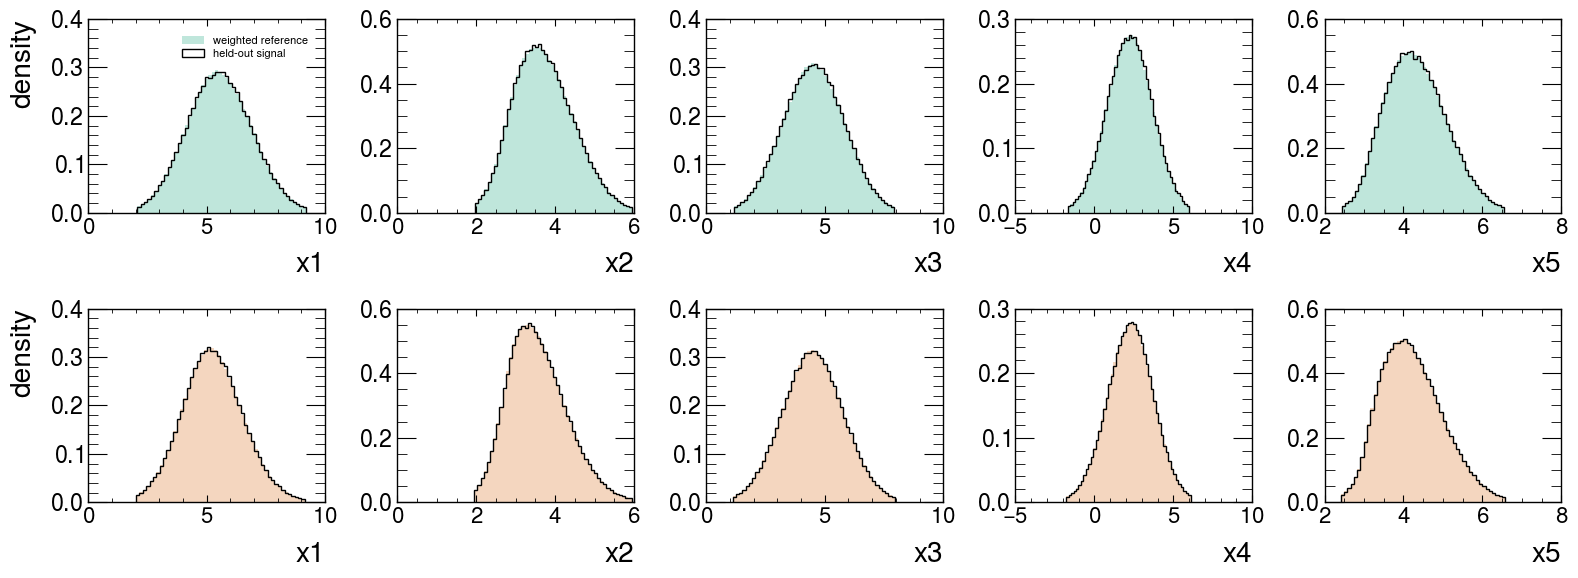
\includegraphics[width=0.98\textwidth]{figures/hybrid_reweighting_closure.png}
  \caption{Process-to-reference ratio closure after preselection.  The five reconstructed features of the five-million-event flow reference are reweighted with $\widetilde r_S^\psi$ (top) and $\widetilde r_B^\psi$ (bottom) and compared with independent selected process samples.  Curves are normalized densities; this test probes the learned ratios independently of the physical $B/S$ normalization.}
  \label{fig:hybrid-closure}
\end{figure}

\subsection{Inference, Asimov dataset, and toys}

The post-selection measurement has one POI, the signal strength $\mu$, with intensity given by \cref{eq:mu-model}.  A JAX-differentiable extended negative log likelihood is minimized with Minuit under $\mu\geq0$.  On the same independent, finite weighted validation measure, the hybrid and analytic reconstructed densities give $\muhat=1.2504$ and $1.1910$, respectively.  The shift attributable to the learned model on this measure is therefore $0.0594$, small compared with the expected statistical uncertainty of approximately $0.56$ but still visible in the profile scan in \cref{fig:inference-results}.  Quoting both minima avoids confusing finite validation-quadrature fluctuation with neural-model bias.

The five-million-event reference sample is converted into the weighted Asimov dataset at $\mu_A=1$.  Its total weight is $153434.077655$, agreeing with $\lambda_S+\lambda_B$ within $2.0\times10^{-10}$.  The analytic score at the generating point is $6.8\times10^{-13}$ and the fit returns $\widehat\mu_A=1.00000000$.  We obtain
\begin{equation}
  q_{0,A}=3.229623,
  \qquad Z_A=1.7971,
  \qquad \sigma_A=0.556447.
  \label{eq:exercise5-asimov}
\end{equation}
A local-curvature estimate gives $0.558017$, a relative difference of $0.28\%$.

Finally, $1000$ pseudo-experiments are generated at each of $\mu=0$ and $\mu=1$.  Independent Poisson signal and background counts are drawn, and reference indices are sampled with probabilities proportional to the normalized component ratios.  At $\mu=1$, the mean fitted signal strength is $1.0156$ and its standard deviation is $0.5217$; the mean observed-information estimate predicts $0.5580$.  The physical-boundary probability is $3.1\%$ in toys, compared with the Asimov/Wald prediction of $3.62\%$.  The right panels of \cref{fig:inference-results} show that the Asimov prediction describes both the estimator width and the boundary-aware $q_0$ distribution at the precision of this toy ensemble.

\begin{figure}[t]
  \centering
  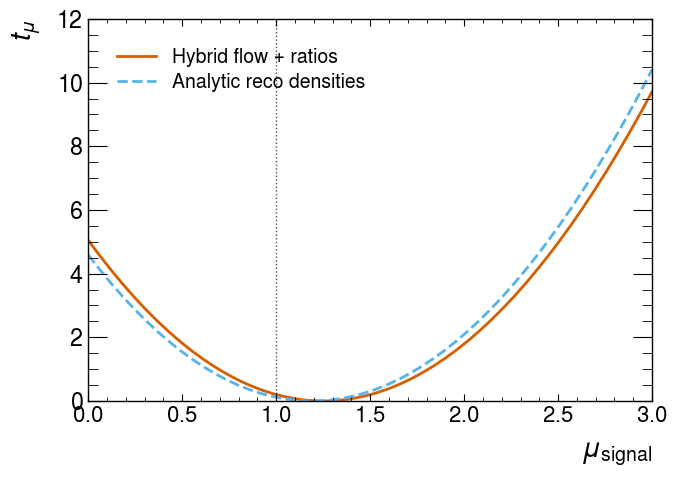
\includegraphics[width=0.34\textwidth]{figures/hybrid_profile.png}
  \hfill
  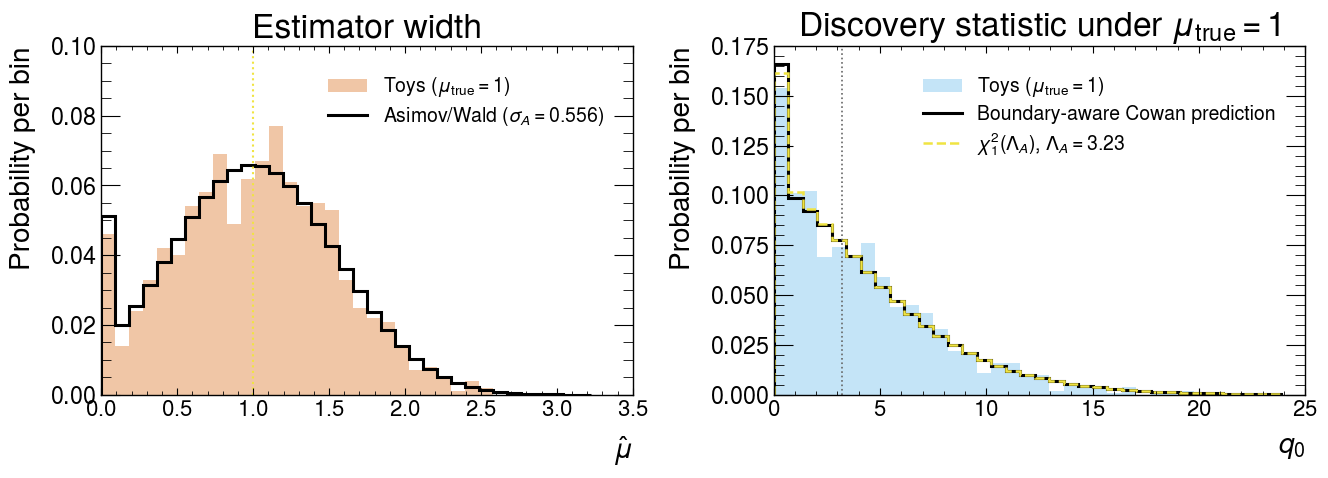
\includegraphics[width=0.63\textwidth]{figures/asimov_toys.png}
  \caption{Inference-level validation.  Left: hybrid and analytic profile-likelihood scans on the same finite validation measure.  Center: the fitted signal-strength distribution for $1000$ pseudo-experiments generated at $\mu=1$, compared with the weighted-Asimov/Wald prediction.  Right: the corresponding discovery statistic compared with the boundary-aware Cowan prediction and an ordinary noncentral $\chi^2$ distribution.  The weighted Asimov fit itself closes exactly at $\mu_A=1$.}
  \label{fig:inference-results}
\end{figure}

\begin{table}[t]
  \caption{Principal Exercise~5 results.  Hybrid and analytic validation fits use the same finite weighted evaluation measure.}
  \label{tab:results}
  \centering
  \begin{tabular}{lc}
    \toprule
    Quantity & Value \\
    \midrule
    Post-selection $(\lambda_S,\lambda_B)$ & $(611.60,152822.48)$ \\
    Raw $(\E_{\qRef}[r_S^\psi],\E_{\qRef}[r_B^\psi])$ & $(0.999149,0.999138)$ \\
    Validation $(\muhat_{\mathrm{hybrid}},\muhat_{\mathrm{truth}})$ & $(1.2504,1.1910)$ \\
    Weighted-Asimov $\widehat\mu_A$ & $1.00000000$ \\
    $(q_{0,A},Z_A)$ & $(3.229623,1.7971)$ \\
    Asimov $\sigma_A$ & $0.556447$ \\
    Toy $\operatorname{std}(\muhat)$ at $\mu=1$ & $0.521740$ \\
    \bottomrule
  \end{tabular}
\end{table}

\subsection{Neural importance-sampling experiment}

Exercise~6 freezes and reloads the reference flow and ratio ensembles from Exercise~5.  A pilot sample of $750000$ points is drawn from $\qRef$.  The scan amplitude in \cref{eq:optimal-scan-proposal} is evaluated at 13 equally spaced values over $0\leq\mu\leq3$, using equal $a_k$ and dividing every $Y_{\mu_k}$ by the total Asimov yield.  The amplitude is floored at $10^{-3}$ of its median positive value and clipped at its $99.9$th percentile.  A sample of $500000$ pilot points, resampled in proportion to this amplitude, trains a smaller quadratic-spline flow with eight coupling layers, three hidden layers of 512 nodes, 16 bins, and tail bound five.  The final proposal uses $\epsilon=0.10$ in \cref{eq:defensive-mixture}.

On $200000$ independent reference points, the centered correlation between $\log A$ and $\log(g_\eta/\qRef)$ is $0.645$, with RMSE $0.268$.  Proposal learning is therefore useful but imperfect, so exact defensive-mixture weights remain essential.  After reweighting, all five reference projections close, as shown in \cref{fig:nis-validation}; the defensive-proposal effective sample size is $183263/200000=91.6\%$.  The $99.9$th percentile of $\qRef/g_\epsilon$ is $3.57$, and its observed maximum is bounded by $10$, as required by $\epsilon=0.10$.

\begin{figure}[t]
  \centering
  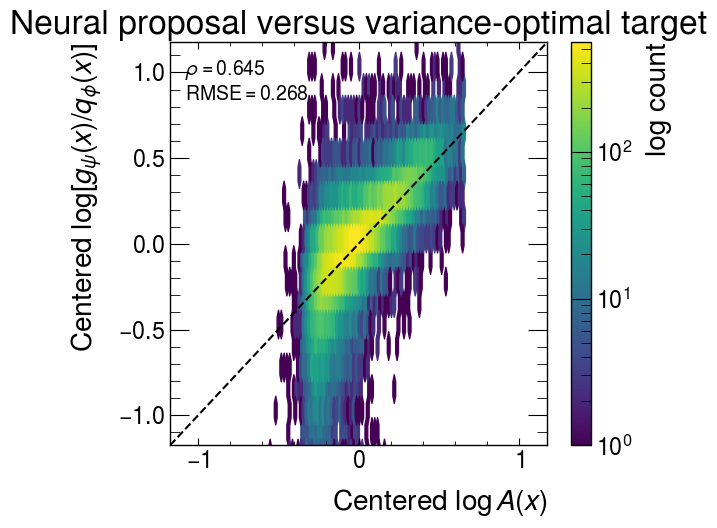
\includegraphics[width=0.35\textwidth]{figures/nis_proposal.png}
  \hfill
  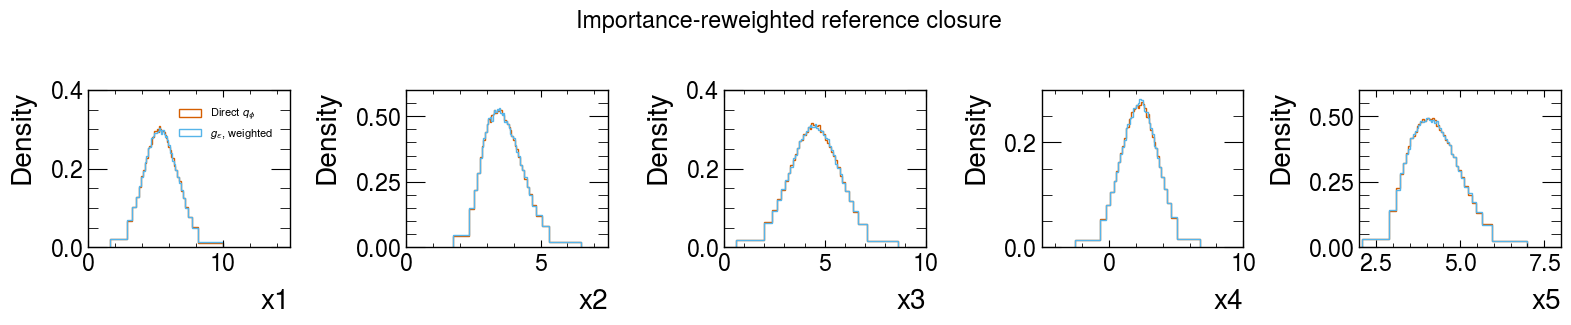
\includegraphics[width=0.62\textwidth]{figures/nis_reweighting.png}
  \caption{Validation of the neural importance proposal.  Left: the learned density displacement $\log(g_\eta/\qRef)$ compared with the scan-amplitude target $\log A$, after subtracting their respective means.  Right: direct reference-flow projections compared with samples from the defensive proposal reweighted by $\qRef/g_\epsilon$.  Exact reweighting restores the reference distribution despite imperfect proposal learning.}
  \label{fig:nis-validation}
\end{figure}

A direct-flow sample of one million events defines a high-statistics benchmark, $q_{0,A}=3.227081\pm0.002568$ from ten blocks and $\sigma_A=0.556666$.  Direct and neural-importance quadratures are then compared at seven sizes from 512 to 32768, using 24 independent repetitions at every size and a 61-point scan over $0\leq\mu\leq3$.  Every quadrature normalizes the signal and background ratios according to \cref{eq:nis-ratio-normalization}, so the maximum absolute score at $\mu_A$ is $1.8\times10^{-12}$ even for the smallest samples.

At the representative size $M=2048$, the RMSE of $q_{0,A}$ decreases from $0.05954$ for direct flow sampling to $0.03658$ for NIS.  The corresponding variance ratio is $2.69$, which can be interpreted as the approximate direct-sampling event factor needed to reach the same precision.  The RMS error over the complete likelihood scan decreases from $0.08548$ to $0.05218$, a reduction of $39\%$.  The gain is largest at intermediate sample sizes and approaches unity when the residual benchmark and repetition precision become limiting, as visible in \cref{fig:nis-performance}.  This experiment demonstrates variance reduction at equal numbers of likelihood-model evaluations; production studies should additionally account for proposal-training and sampling wall time.

\begin{figure}[t]
  \centering
  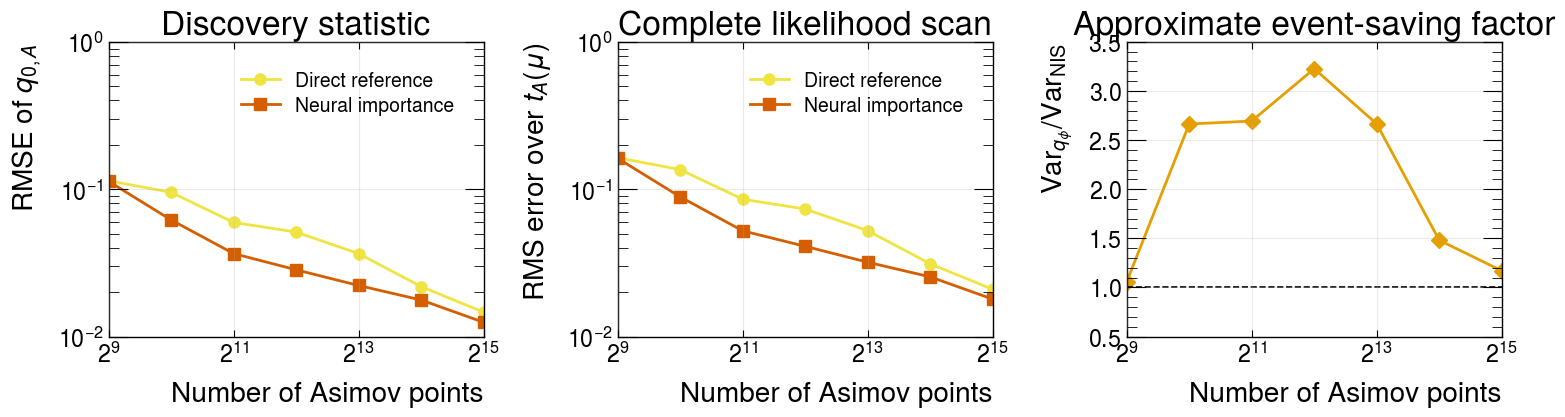
\includegraphics[width=0.98\textwidth]{figures/nis_convergence.png}
  \caption{Equal-size Asimov quadrature comparison over 24 repetitions.  Left: RMSE of the discovery statistic relative to the million-event benchmark.  Center: RMS error of the complete expected likelihood-ratio scan.  Right: ratio of the direct-reference variance to the neural-importance variance.  At $M=2048$, the variance reduction is $2.69$ and the complete-scan RMSE is reduced by $39\%$.}
  \label{fig:nis-performance}
\end{figure}

\section{Discussion and outlook}
\label{sec:discussion}

Hybrid NSBI changes the role of absolute density estimation.  Training an independent flow for every sample asks each model to be accurate enough that the ratio of two imperfect densities supports a precision measurement.  The hybrid approach asks one flow to cover the combined reference phase space and learns every precision-critical correction discriminatively.  Because the denominator events are drawn from that trained flow, classifier ratios correct its local density distortions in the population limit.  At the same time, the explicit $\qRef$ factor turns the ratio representation into a normalized density model.

This construction addresses both operational limitations in \cref{sec:ratio-limitations}.  The flow can generate arbitrarily many independent reference points, so numerical quadrature for profiles, impacts, and Asimov calculations is not capped by the original MC.  The normalized ratios turn the same proposal into process-specific samplers, enabling pseudo-experiments and Neyman constructions without a separate generative model for every parameter point.  NIS adds a distinct efficiency layer: it concentrates the Asimov quadrature where the expected scan receives its largest event-level contributions, while exact weights retain the frozen hybrid model.

Several limitations remain and should be treated as part of the method definition.
\begin{itemize}
  \item \emph{Support and importance-weight variance.}  A flow that misses a relevant region creates extreme ratios and low effective sample size.  Balanced-mixture design, tail modeling, ratio-tail monitoring, and sample-wise effective sample sizes are mandatory diagnostics.
  \item \emph{Classifier misspecification.}  Finite normalization fixes only the integral.  Calibration, reweighting, ensemble stability, and inference-level closure against independent samples remain necessary.  Neyman construction is especially valuable when residual neural bias could invalidate simple asymptotic assumptions.
  \item \emph{Finite quadrature.}  Yield normalization guarantees stationarity at the generating point but not an exact expected scan away from it.  Block errors, repeated quadratures, and direct-versus-importance comparisons are needed to quantify numerical integration uncertainty separately from flow and classifier bias.
  \item \emph{Task-specific NIS.}  The optimal proposal depends on the selected scan and loss weights.  A proposal trained only for $q_0$ may be inefficient for distant interval crossings or nuisance impacts.  The design grid must cover the downstream statistical task, and the reference component must remain in the defensive mixture.
  \item \emph{Negative-weight and interference components.}  Individual signed contributions are not probability densities and cannot be sampled directly.  A practical implementation must use positive physical combinations as sampling channels while retaining analytic signed coefficients in the intensity, as is already done in semi-parametric NSBI.
  \item \emph{Nuisance-parameter coverage.}  A nominal reference must cover the support of all relevant systematic variations.  Very large shape changes may require a broader mixture or a conditional reference flow.
\end{itemize}

The reference and integration proposals serve different objectives.  Equal sample normalization is a robust choice for $\qRef$ because it supports ratio training and generation for every component.  The neural importance flow is instead optimized for a chosen statistical calculation and can be retrained without changing the likelihood model.  One NIS target may cover a POI scan, several nuisance-profile trajectories, or a set of impact calculations through the weights $a_k$.  For high-dimensional problems, mixtures of flows, heavier-tailed bases, or iterative proposals may be preferable.

The flow map also permits RQMC points to be transported from the latent base distribution.  This strategy is complementary to NIS: the latter reshapes the sampling density, whereas RQMC improves space filling within that density.  Their combination is a natural next step, provided uncertainty is assessed with independent scramblings rather than an i.i.d. standard-error formula.  More broadly, developments in conditional or non-parametric NSBI can be incorporated at the ratio layer without changing the tractable reference and integration machinery.

\section{Conclusion}
\label{sec:conclusion}

We have introduced hybrid neural simulation-based inference, a construction that combines a tractable normalizing-flow reference with classifier estimates of sample-to-reference density ratios.  Sampling the denominator class from the learned flow makes each ratio a correction to that specific tractable proposal, so local flow error cancels in the ideal classifier limit.  The resulting sample densities can be evaluated, integrated, and sampled while inference retains the ratio structure of semi-parametric NSBI.

The hybrid representation supplies two statistical objects that are cumbersome in a ratio-only analysis: a weighted unbinned Asimov measure and a process sampler for pseudo-experiments.  Matching the total Asimov weight to the expected yield supplies the extended term, and component normalization on the same quadrature guarantees exact finite-sample stationarity for yield parameters.  In the demonstration, the Asimov fit closes at $\mu_A=1$, and its $q_{0,A}$ predicts the estimator width and boundary-aware toy distribution observed in 1000 pseudo-experiments.

Finally, we formulated the expected test-statistic scan as a set of integrals and trained a second flow toward their variance-optimal proposal.  At 2048 quadrature points, this neural importance sampler reduces the $q_{0,A}$ variance by a factor of $2.69$ and the full-scan RMSE by $39\%$.  The reference flow therefore makes an Asimov calculation cheap and renewable; neural importance sampling makes it efficient.  Together they preserve the central advantage of semi-parametric NSBI---precision corrections learned as density ratios---while adding the tractable integration and generation needed for standard LHC statistical workflows.

\begin{acknowledgments}
We would like to thank the organizers of the 2026 ML4HEP School at the Tata Institute of Fundamental Research, where the initial idea for this project was developed, and the US National Science Foundation HSF-India OISE-2201990 for support during the school.  The work of RCLSA is partially supported by the US Department of Energy award DE-SC0010004.
\end{acknowledgments}

\bibliography{references}

\end{document}
